\documentclass[11pt]{article}
\usepackage[margin=0cm,nohead]{geometry}
\usepackage[active,tightpage]{preview}

\usepackage{transparent}

\usepackage[scr,scaled=1.1]{rsfso}

\usepackage{tikz,amsmath,amssymb,mathtools,bm,color,cancel}

%\usepackage{newtxtext}
%\usepackage{newtxmath}

\usetikzlibrary{shapes,arrows}
\usetikzlibrary{calc}
\usetikzlibrary{positioning}
\usetikzlibrary{decorations.pathreplacing}

\PreviewEnvironment{tikzpicture}
\setlength\PreviewBorder{-1mm}

\begin{document}

\begin{tikzpicture}

%%%%%%%%%%%%%%%%%%%%%%%%%%%%%%%%%%%%%%%%%%%%%%%%%%%%%%%%%%%%%% Macros

\newcommand{\tr}{\mathsf{{\scriptscriptstyle T}}}
\newcommand{\ii}{\mathrm{i}}
\newcommand{\ee}{\operatorname{e}}
\newcommand{\dd}{\mathrm{d}}
\newcommand{\op}[1]{\operatorname{#1}}

\newcommand{\pL}{\mathsf{{\scriptscriptstyle L}}}
\newcommand{\pR}{\mathsf{{\scriptscriptstyle R}}}
\newcommand{\pC}{\mathsf{{\scriptscriptstyle C}}}

\newcommand{\bPsi}{\boldsymbol{\Psi}}
\newcommand{\bPhi}{\boldsymbol{\Phi}}

\newcommand{\suY}{\mathrm{\scriptscriptstyle Y}}
\newcommand{\suL}{\mathrm{\scriptscriptstyle L}}
\newcommand{\suC}{\mathrm{\scriptscriptstyle C}}

\newcommand{\dbar}[1]{\overline{#1}}
\newcommand{\sbar}[1]{\bar{#1}}
\newcommand{\anti}[1]{\bar{#1}}

\newcommand{\quantNo}[3]{\mathbf{#1},\mathbf{#2},#3}
 
%%%%%%%%%%%%%%%%%%%%%%%%%%%%%%%%%%%%%%%%%%%%%%%%%%%%%%%%%%%%%% Styles

\tikzset{myRow/.style     ={draw,anchor=north west,rectangle}}
\tikzset{boxNone/.style   ={anchor=north west}}
\tikzset{boxWhite/.style  ={draw,anchor=north west,rectangle, very thin, rounded corners=5pt, fill=white}}
\tikzset{boxGray/.style   ={draw,anchor=north west,rectangle, very thin, rounded corners=5pt, fill=gray!10}}
\tikzset{boxRed/.style    ={draw,anchor=north west,rectangle, very thin, rounded corners=5pt, fill=red!4}}
\tikzset{boxGreen/.style  ={draw,anchor=north west,rectangle, very thin, rounded corners=5pt, fill=green!4}}
\tikzset{boxYellow/.style ={draw,anchor=north west,rectangle, very thin, rounded corners=5pt, fill=yellow!5}}
\tikzset{boxBlue/.style   ={draw,anchor=north west,rectangle, very thin, rounded corners=5pt, fill=blue!4}}
\tikzset{boxCyan/.style   ={draw,anchor=north west,rectangle, very thin, rounded corners=5pt, fill=cyan!2}}
\tikzset{colorLagr/.style ={fill=magenta!8}}
\tikzset{arr/.style       ={->}}
\tikzset{circled/.style   ={fill=black!60!blue,thin,circle,inner sep=2.5pt}}

%%%%%%%%%%%%%%%%%%%%%%%%%%%%%%%%%%%%%%%%%%%%%%%%%%%%%%%%%%%%%% Row/Column styles

\tikzset{R/.style={
	minimum height = #1 mm
}}

\tikzset{C/.style={
    minimum width = #1 mm, 
    text width = #1 mm - 3 mm,
    inner sep = 5
}}

%%%%%%%%%%%%%%%%%%%%%%%%%%%%%%%%%%%%%%%%%%%%%%%%%%%%%%%%%%%%%% Paper W/H

\node at (-20.5,14.5) {}; \node at (20.35,-14.5) {};

%%%%%%%%%%%%%%%%%%%%%%%%%%%%%%%%%%%%%%%%%%%%%%%%%%%%%%%%%%%%%% Title

\node [color=black] at (0,14.25) {
	\huge\sf Tangent Spaces, Overview
};

\node [anchor=north, color=black] at (0,13.9) {
	by M.B.Kocic ~--~ Version 1.02 (2017-06-03) ~--~ Advanced GR
	~--~ (partly based on F.P.\;Schuller's lectures, WE-Heraeus, 2015)
};

\pdfinfo {
%	/CreationDate	(D:20160121124500)
	/Title			(Tangent Spaces)
	/Author			(Mikica B Kocic)
	/Subject		(Advanced GR RC)
	/Keywords		(GR)
	/Creator		(TeX-TikZ)
}

%%%%%%%%%%%%%%%%%%%%%%%%%%%%%%%%%%%%%%%%%%%%%%%%%%%%%%%%%%%%%%

\node [rotate=50] at (-16.25,6.25) {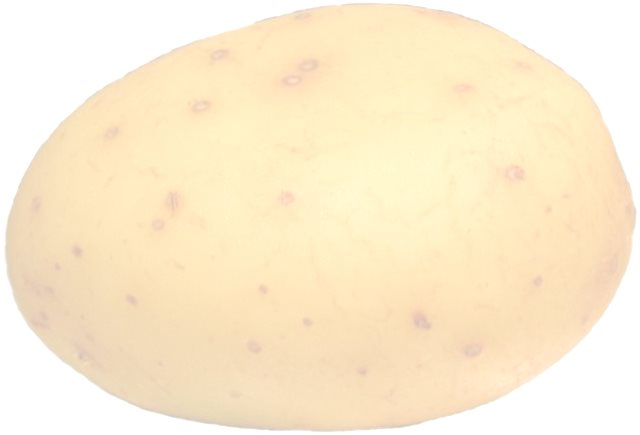
\includegraphics[width=60mm]{potato.jpg}};

\node [boxRed,colorLagr,R=10,C=100] at (-20.5,13) {
	\hspace{12mm} \textsf{The velocity of a curve $\gamma$ at a point $p\in\mathscr{M}$.}
};

\node [boxNone,C=100] at (-20.5,11.75) {
	Let $(\mathscr{M},\mathscr{O},\mathscr{A})$ be a smooth manifold with
	a topology $\mathscr{O}$ and a smooth atlas $\mathscr{A}$.
	Let further,\vspace{-2mm}
	\[
		\gamma : \mathbb{R} \to \mathscr{M},\vspace{-3mm}
	\]
	be at least $C^1$ smooth curve on $\mathscr{M}$
	parameterized by $\lambda \mapsto \gamma(\lambda)$.
};

\node [boxNone,C=50] at (-15.25,4.5) {
	\small To determine velocity, we\\[-1pt]
	must have a test scalar field.
};

\node [boxYellow,C=100] at (-20.5,3) {
	The \emph{velocity of a curve $\gamma$ at a point
	$p\in\mathscr{M}$} is the \textbf{linear map},\vspace{-2mm}
	\[
		v_{\gamma,p}:C^{\infty}(\mathscr{M}) \to \mathbb{R},
		\vspace{-2mm}
	\]
	defined by,\vspace{-4mm}
	\[
		f \mapsto v_{\gamma,p}(f) \coloneqq ( f \circ \gamma )^\prime (\lambda_0),
		\vspace{-3mm}
	\]
	where $p = \gamma(\lambda_0).$
};

\node (d1-M) at (-15.5,-0.75) {$\mathscr{M}$};
\node (d1-R1) at (-18,-0.75) {$\mathbb{R}$};
\node (d1-R2) at (-13,-0.75) {$\mathbb{R}$};

\draw [arr] (d1-R1) edge node[above] {$\gamma$} (d1-M);
\draw [arr] (d1-M) edge node[above] {$f$} (d1-R2);
\draw [arr] (d1-R1) edge [bend right=25] node[xshift=0,yshift=-7] {$f\circ\gamma$} (d1-R2);

\node [boxNone,C=100] at (-20.5,-2.25) {
	Here, $C^{\infty}(\mathscr{M})$ is the vector space of 
	smooth functions on the manifold $\mathscr{M}$,\vspace{-2mm}
	\[
		C^{\infty}(\mathscr{M}) \coloneqq 
		\{ f : \mathscr{M} \to \mathbb{R} \ \vert\ \text{$f$ is smooth} \}.
		\vspace{-2mm}
	\]
	Note:
	$(f+g)(p)\coloneqq v(p)+g(p)$, 
	$(\alpha\cdot f)(p) \coloneqq \alpha \cdot f(p)$.
};

\node [boxRed,colorLagr,R=10,C=100,align=center] at (-20.5,-5) {
	\textsf{Tangent space, intrinsic definition}
};

\node [boxYellow,C=100] at (-20.5,-6) {
	The \emph{tangent space to $\mathscr{M}$ at $p$}, 
	denoted by $T_p\mathscr{M}$, is the \textbf{set} of the velocities of all
	smooth curves in $\mathscr{M}$ passing through $p$,
	\vspace{-2mm}
	\[
		T_p\mathscr{M} \coloneqq
		\{ v_{\gamma,p} \ \vert\ \text{$\gamma$ is smooth} \}.
	\]
};

\node [boxNone,C=100] at (-20.5,-8.5) {
	Define two binary operations on $T_p\mathscr{M}$,\vspace{-2mm}
	\[
		(v_{\gamma,p} + v_{\delta,p})(f) \coloneqq
		v_{\gamma,p}(f) + v_{\delta,p}(f),\vspace{-2mm}
	\]
	\[
		(\alpha \cdot v_{\gamma,p})(f) \coloneqq
		\alpha \cdot v_{\gamma,p}(f),
	\]
	where $v_{\gamma,p},v_{\delta,p}\in T_p\mathscr{M}$
	and $\alpha\in\mathbb{R}$.
};

\node [boxBlue,R=10,C=100] at (-20.5,-11.5) {
	Proposition. $T_p\mathscr{M}$ equipped with $+$ and $\cdot$
	from above is a \textbf{vector space}.
};

\node [boxNone,C=100] at (-20.5,-12.75) {
	Proof by construction (in an arbitrary chart). E.g.,\\
	$(x\circ\sigma)(\lambda) =
	(x\circ\gamma)(\lambda_0+\lambda) +
	(x\circ\delta)(\lambda_1+\lambda) -
	(x\circ\gamma)(\lambda_0)
	$\\
	where $p=\gamma(\lambda_0)=\delta(\lambda_1)$.
};


%%%%%%%%%%%%%%%%%%%%%%%%%%%%%%%%%%%%%%%%%%%%%%%%%%%%%%%%%%%%%%

\node [rotate=50] at (-7,6.25) {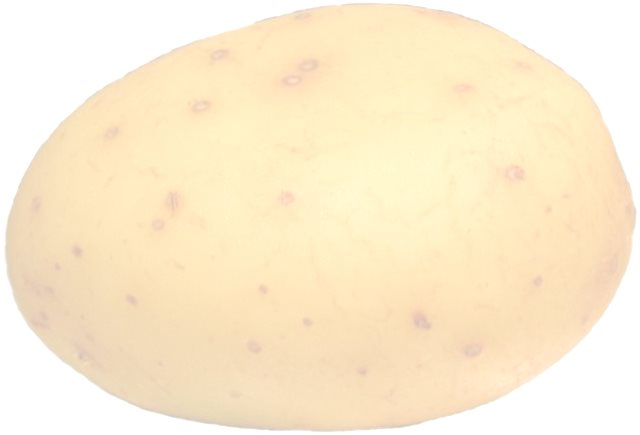
\includegraphics[width=60mm]{potato.jpg}};

\node [boxRed,colorLagr,R=10,C=100] at (-10.25,13) {
	\hspace{8mm} \textsf{The components of a vector $\in T_p\mathscr{M}$ wrt a chart.}
};

\node (d2-M) at (-5.5,-1.5) {$\mathscr{M}$};
\node (d2-R1) at (-8.5,-1.5) {$\mathbb{R}$};
\node (d2-R2) at (-2.5,-1.5) {$\mathbb{R}$};
\node [blue] (d2-Rm1) at (-5.5,-4.5) {$\mathbb{R}^m$};

\node [rotate=90,blue] (d2-U1) at (-5.5,-2.25) {$\mathscr{U}\subseteq$};

\draw [arr,thick] (d2-R1) edge node[above] {$\gamma$} (d2-M);
\draw [arr,thick] (d2-M) edge node[above] {$f$} (d2-R2);

\draw [arr,blue] (d2-U1) edge node[right,yshift=4] {$x$} (d2-Rm1);

\draw [arr] (d2-R1) edge [bend left=30] node[above] {$f\circ\gamma$} (d2-R2);

\draw [arr,blue] (d2-R1) edge node[xshift=-15,yshift=-5] {$x\circ\gamma$} (d2-Rm1);
\draw [arr,blue] (d2-Rm1) edge node[xshift=17,yshift=-5] {$f\circ x^{-1}$} (d2-R2);

\node [boxNone,C=50,blue,rotate=90] at (-1.75,-4.65) {\small Representatives\\[-2pt]in the chart $(\mathscr{U_x},x)$};
\draw [blue,decorate, decoration={brace, amplitude=7pt}](-2,-1.75) -- (-2,-4.5);

%%%%%%%%%%%%%%%%%%%%%%%%%%%%%%%%%%%%%%%%%%%%%%%%%%%%%%%%%%%%%%

\node [rotate=50] at (3.25,6.5) {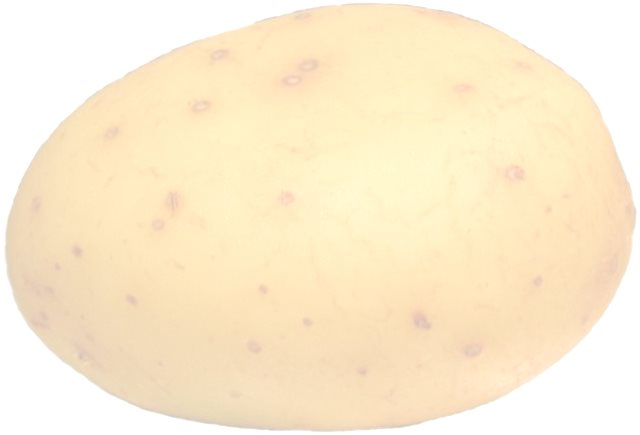
\includegraphics[width=60mm]{potato.jpg}};

\node [boxRed,colorLagr,R=10,C=100,align=center] at (0,13) {
	~\textsf{Change of vector components under a change of chart.}
};

\node [boxNone,C=100] at (0,11.75) {
	Let $(\mathscr{U}_x,x)$ and $(\mathscr{U}_y,y)$ be two charts from the
	atlas $\mathscr{A}$,
	such that,\vspace{-2mm}
	\[
	p = \gamma(\lambda_0) \in \mathscr{U},\vspace{-1mm}
	\]
	where $\mathscr{U}= 
	\mathscr{U}_x \cap \mathscr{U}_y  \subseteq\mathscr{M}$.
};

\node (d3-M) at (4,-1) {$\mathscr{M}$};
\node (d3-R1) at (1,-1) {$\mathbb{R}$};
\node (d3-R2) at (7,-1) {$\mathbb{R}$};
\node [blue] (d3-Rm1) at (4,-4) {$\mathbb{R}^m$};
\node [red] (d3-Rm2) at (4,2) {$\mathbb{R}^m$};

\node [rotate=90,blue] (d3-U1) at (4,-1.75) {$\mathscr{U}_x\subseteq$};
\node [rotate=-90,red] (d3-U2) at (4,-0.25) {$\mathscr{U}_y\subseteq$};

\draw [arr,thick] (d3-R1) edge node[above] {$\gamma$} (d3-M);
\draw [arr,thick] (d3-M) edge node[above] {$f$} (d3-R2);

\draw [arr,blue] (d3-U1) edge node[right] {$x$} (d3-Rm1);
\draw [arr,red] (d3-U2) edge node[right] {$y$} (d3-Rm2);

\draw [arr] (d3-R1) edge [bend right=22] node[xshift=38,yshift=-3,rotate=18] {$f\circ\gamma$} (d3-R2);

\draw [arr,blue] (d3-R1) edge node[xshift=-15,yshift=-5] {$x\circ\gamma$} (d3-Rm1);
\draw [arr,blue] (d3-Rm1) edge node[xshift=17,yshift=-5] {$f\circ x^{-1}$} (d3-R2);
\draw [arr,red] (d3-R1) edge node[xshift=-15,yshift=5] {$y\circ\gamma$} (d3-Rm2);
\draw [arr,red] (d3-Rm2) edge node[xshift=15,yshift=8] {$f\circ y^{-1}$} (d3-R2);
\draw [arr,green!50!black] (d3-Rm1) edge [bend left=25] node[xshift=-3,yshift=33,rotate=75] {$y\circ x^{-1}$} (d3-Rm2);

\node [blue] at (-2.5,8) {\small Chart representatives:};

\draw [dashed,green!50!black](3.4983,0.8857) -- (2.6175,1.5781);
\node [C=50,green!50!black] at (3,2) {\small Chart\\[-1mm]transition map};


\node [boxNone,C=100] at (0,-4.5) {
	Consider a vector $V_p \in T_p\mathscr{M}$.
	Then, there are unique components $V^\mu_{(x),p}$ and $V^\mu_{(y),p}$ 
	in the chart induces bases with respect to 
	$(\mathscr{U}_x,x)$ and $(\mathscr{U}_y,y)$,
	such that,\vspace{-2mm}
	\[
		V_p = V^\mu_{(x),p} \left( \frac{\partial}{\partial x^\mu} \right)_p 
		= V^\nu_{(y),p} \left( \frac{\partial}{\partial y^\nu} \right)_p.
		\vspace{-2mm}
	\]
	But, $ \left( \frac{\partial f}{\partial x^\mu} \right)_p $
	$ = \partial_\mu(f \circ x^{-1})\left( x(p) \right) $\\\qquad 
	$ = \partial_\mu\left((f \circ y^{-1}) \circ (y \circ x^{-1}) \right)
	\left( x(p) \right) $\\\qquad 
	$ = \partial_\mu(y^\nu \circ x^{-1}) \left( x(p) \right) \cdot 
	\partial_\nu(f \circ y^{-1}) \left( y(p) \right) $\\\qquad 
	$ = \left( \frac{\partial y^\nu}{\partial x^\mu} \right)_p
	\left( \frac{\partial f}{\partial y^\nu} \right)_p $,\\[2mm]
	so that:
	$
		V^\mu_{(x),p} \left( \frac{\partial y^\nu}{\partial x^\mu} \right)_p
		\left( \frac{\partial f}{\partial y^\nu} \right)_p 
		= V^\nu_{(y),p} \left( \frac{\partial}{\partial y^\nu} \right)_p
	$.\\Therefore,
};

\node [boxGreen,R=15,C=50,align=center] at (2.5,-11.25) {
	$\displaystyle
	 V^\nu_{(y),p} 
	 = V^\mu_{(x),p} \left( \frac{\partial y^\nu}{\partial x^\mu} \right)_p
	$
};

%%%%%%%%%%%%%%%%%%%%%%%%%%%%%%%%%%%%%%%%%%%%%%%%%%%%%%%%%%%%%%

\node [rotate=50] at (14.25,5) {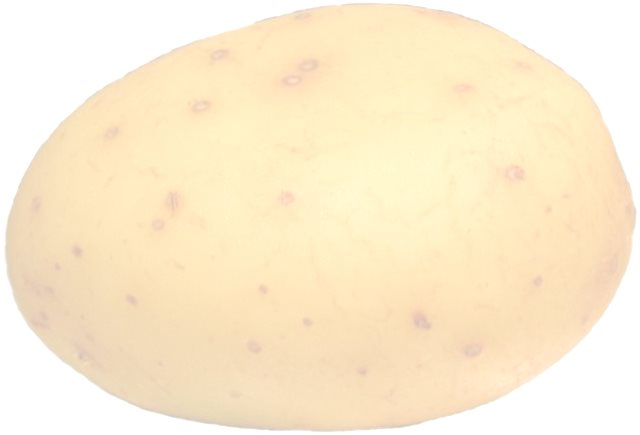
\includegraphics[width=60mm]{potato.jpg}};

\node [boxRed,colorLagr,R=10,C=100,align=center] at (10.25,13) {
	~\textsf{Change of vector components under a pushforward.}
};

\node [boxNone,C=100] at (10.25,11.75) {
	Let $\varphi : \mathscr{M} \to \mathscr{N}$ be a smooth map 
	between manifolds. 
	Let further $g:\mathscr{N}\to\mathbb{R}$ be 
	a smooth function on $\mathscr{N}$. \\
	\quad Then the \emph{pullback of
	the function $g$ by $\varphi$} to $p\in\mathscr{M}$ is 
	the precomposition of $g$ by $\varphi$ at $p$,
	\vspace{-2mm}
	\[
		(\varphi^{*} g)(p) \coloneqq (g \circ \varphi)(p) 
		= g \left( \varphi(p) \right) = g(q),
		\vspace{-2mm}
	\]
	where $q=\varphi(p)\in\mathscr{N}$.
};

\node [blue] (d4-M) at (13.5,-3.75) {$\mathscr{M}$};
\node [red] (d4-N) at (17,-3.75) {$\mathscr{N}$};
\node (d4-R1) at (11.5,-1.75) {$\mathbb{R}$};
\node (d4-R2) at (19,-1.75) {$\mathbb{R}$};
\node [blue] (d4-Rm1) at (13.5,-7.25) {$\mathbb{R}^m$};
\node [red] (d4-Rn) at (17,-7.25) {$\mathbb{R}^n$};

\node [rotate=90,blue] (d4-U1) at (13.5,-4.6) {$\mathscr{U}_x\subseteq$};
\node [rotate=-45,blue] (d4-U3) at (14.2,-4.45) {$\supseteq\mathscr{U}_z$};
\node [rotate=90,red] (d4-V) at (17,-4.5) {$\mathscr{V}_z\subseteq$};

\draw [arr,thick] (d4-R1) edge node[right] {$\gamma$} (d4-M);
\draw [arr,thick] (d4-M) edge node[xshift=4,yshift=9,rotate=19.5] {$f=\varphi^{*}g\coloneqq g\circ\varphi$} (d4-R2);

\draw [arr,blue] (d4-U1) edge node[right] {$x$} (d4-Rm1);

\draw [arr] (d4-R1) edge node[below] {$f\circ\gamma$} (d4-R2);

\draw [arr,blue] (d4-R1) edge [bend right=22] node[left] {$x\circ\gamma$} (d4-Rm1);
\draw [arr,red] (d4-Rn) edge [bend right=22] node[right] {$g\circ z^{-1}$} (d4-R2);
\draw [arr,blue] (d4-Rm1) edge [bend right=25] node[xshift=29,yshift=25,rotate=56] {$f\circ x^{-1}$} (d4-R2);

\draw [arr,thick] (d4-M) edge node[below] {$\varphi$} (d4-N);
\draw [arr,blue] (d4-U3) edge node[xshift=-3,yshift=11] {$\hat{z}$} (d4-Rn);
\draw [arr,red] (d4-V) edge node[right] {$z$} (d4-Rn);
\draw [arr,thick,red] (d4-N) edge node[right] {$g$} (d4-R2);
\draw [arr,green!50!black] (d4-Rm1) edge node[below] {$\hat{z}\circ x^{-1}$} (d4-Rn);

\node [boxYellow,C=100] at (10.25,1.25) {
	Let $V_p$ be a vector in $T_p\mathscr{M}$.
	Then the \emph{pushforward of $V_p$ by $\varphi$} to $T_q\mathscr{N}$ 
	(to act on $g\in C^\infty(\mathscr{N})$)
	is the composition of $V_p$ with the pullback of $g$ by $\varphi$,
	\vspace{-2mm}
	\[
		(\varphi_{*} V_p)(g) \coloneqq V_p \left( \varphi^{*}g \right)
		= V_p\left( g \circ \varphi \right) = V_p(f).
	\]
};

\node [boxNone,C=100] at (10.25,-8) {
	Let $(\mathscr{U}_x,x)$ be a chart on $\mathscr{M}$
	and $(\mathscr{V}_z,z)$ a chart on $\mathscr{N}$, such that
	$\mathscr{U}_x=\mathrm{preim}_\varphi\mathscr{V}_z$
	and	$p\in\mathscr{U}_x$, $q\in\mathscr{V}_z$.\\
	We have, 
	$ \left( \varphi_{*}V_p \right)_q (g) 
		= \left( \varphi_{*}V_p \right)^\alpha_{(z),q} 
		\left( \frac{\partial g}{\partial z^\alpha} \right)_q$, 
		but also:\\
	$\left( \varphi_{*}V_p \right)_q (g)
	= V_p\left( \varphi^{*}g \right) = V_p\left( f \right)$
	$= v_{\gamma,p}(f) = v_{\gamma,p}(g \circ \varphi)$\\ 
	$= \left( g \circ \varphi \circ \gamma \right)^\prime (\lambda_0) 
	= \left( ( g \circ z^{-1} ) \circ ( \hat{z} \circ \gamma ) \right)^\prime (\lambda_0) $ \\
	$= \left( ( g \circ z^{-1} ) \circ ( \hat{z} \circ x^{-1}) \circ 
		( x \circ \gamma ) \right)^\prime (\lambda_0)$\\
	$= \left( x^\mu \circ \gamma \right)^\prime(\lambda_0) 
	\cdot \partial_\mu \left( \hat{z}^\nu \circ x^{-1} \right) \left( x(p) \right) 
	\cdot \partial_\nu \left( g \circ z^{-1} \right) \left( z(q) \right)$
	$= V^\mu_{(x),p} \left( \frac{\partial \hat{z}^\alpha}{\partial x^\mu} \right)_p
	\left( \frac{\partial g}{\partial z^\alpha} \right)_q
	$. ~Hence, 
	$(\varphi_{*})^\alpha_{\ \;\mu} = \left( \frac{\partial \hat{z}^\alpha}{\partial x^\mu} \right)_p$
	and,
};

\node [boxGreen,R=15,C=50,align=center] at (15.25,-13) {
	$\displaystyle
	 \left( \varphi_{*}V_p \right)^\alpha_{(z),q}  
	 = V^\mu_{(x),p} \left( \frac{\partial \hat{z}^\alpha}{\partial x^\mu} \right)_p
	$
};

\node [boxYellow,R=15,C=72] at (7.8,-13) {
	~If $\varphi$ is bijective and $\varphi^{-1}$ is also smooth,\\
	~then $\varphi$ is called a \emph{diffeomorphism}.
};

\node [boxNone,C=72] at (0.5,-13.2) {
	$\bullet$ \textsf{Passive (or alias) transformation}
};

\node [boxNone,C=72] at (0.5,-13.75) {
	$\bullet$ \textsf{Active (or alibi) transformation}
};


\draw [-triangle 45,gray!60] (7.5,-14.15) -- (6.65,-14.15);
\draw [-triangle 45,gray!60] (2.2107,-12.5041) -- (1.7087,-13.0148);

\draw [-triangle 45,gray!60] (19.7524,-12.4619) -- (19.7524,-12.8619);
\draw [-triangle 45,gray!60] (1.6751,-11.5677) -- (2.2453,-11.8819);

%%%%%%%%%%%%%%%%%%%%%%%%%%%%%%%%%%%%%%%%%%%%%%%%%%%%%%%%%%%%%%

% \node [blue] (d5-M) at (15,-10.5) {$\mathscr{M}$};
% \node [red] (d5-N) at (18,-12) {$\mathscr{N}$};
% \node (d5-R1) at (12,-9) {$\mathbb{R}$};
% \node (d5-R2) at (18,-9) {$\mathbb{R}$};
% \node [blue] (d5-Rm1) at (12,-12) {$\mathbb{R}^m$};
% \node [blue] (d5-Rm2) at (15,-7) {$\mathbb{R}^m$};
% \node [red] (d5-Rn) at (15,-14) {$\mathbb{R}^n$};
% 
% \node [rotate=32,blue] (d5-U1) at (14.2457,-10.8936) {$\mathscr{U}_x\subseteq$};
% \node [rotate=-90,blue] (d5-U2) at (15,-9.75) {$\mathscr{U}_y\subseteq$};
% \node [rotate=90,blue] (d5-U3) at (15,-11.25) {$\mathscr{U}_z\subseteq$};
% \node [rotate=40,red] (d5-V) at (17.4282,-12.4043) {$\mathscr{V}\subseteq$};
% 
% \draw [arr,thick] (d5-R1) edge node[xshift=10,yshift=1] {$\gamma$} (d5-M);
% \draw [arr,thick] (d5-M) edge node[xshift=-6,yshift=4,rotate=28] {$f=g\circ\varphi$} (d5-R2);
% 
% \draw [arr,blue] (d5-U1) edge node[xshift=-1,yshift=5] {$x$} (d5-Rm1);
% \draw [arr,blue] (d5-U2) edge node[xshift=-5,yshift=3] {$y$} (d5-Rm2);
% 
% \draw [arr] (d5-R1) edge node[xshift=30,yshift=7] {$f\circ\gamma$} (d5-R2);
% 
% \draw [arr] (d5-R1) edge node[left] {$x\circ\gamma$} (d5-Rm1);
% \draw [arr,green!50!black] (d5-R1) edge node[xshift=-15,yshift=5] {$y\circ\gamma$} (d5-Rm2);
% \draw [arr,green!50!black] (d5-Rm2) edge node[xshift=15,yshift=8] {$f\circ y^{-1}$} (d5-R2);
% \draw [arr,green!50!black] (d5-Rm1) edge [bend right=24] node[xshift=45,yshift=22,rotate=45] {$f\circ x^{-1}$} (d5-R2);
% \draw [arr,green!50!black] (d5-Rm1) edge [bend left=6] node[xshift=12,yshift=30,rotate=52] {$y\circ x^{-1}$} (d5-Rm2);
% 
% \draw [arr,thick] (d5-M) edge node[below] {$\varphi$} (d5-N);
% \draw [arr,blue] (d5-U3) edge node[xshift=5,yshift=3] {$\hat{z}$} (d5-Rn);
% \draw [arr,red] (d5-V) edge node[xshift=3,yshift=-4] {$z$} (d5-Rn);
% \draw [arr,thick] (d5-N) edge node[right] {$g$} (d5-R2);
% \draw [arr,green!50!black] (d5-Rm1) edge node[xshift=-15,yshift=-6] {$\hat{z}\circ x^{-1}$} (d5-Rn);
% 

%%%%%%%%%%%%%%%%%%%%%%%%%%%%%%%%%%%%%%%%%%%%%%%%%%%%%%%%%%%%%%

\draw [thick] (-17.7547,3.7196) .. controls (-17.25,4.75) and (-18.25,5.75) .. (-16.5,6) .. controls (-14.5,6.25) and (-17.25,8.25) .. (-14.7692,8.7142);

\draw [black,fill=black] (-16.5,6) ellipse (0.05 and 0.05);

\node at (-14.3436,7.634) {\Large $\mathscr{M}$};
\node at (-16.4923,5.6015) {$p=\gamma(\lambda_0)$};
\node at (-15.4696,8.1395) {\Large $\gamma$};

%%%%%%%%%%%%%%%%%%%%%%%%%%%%%%%%%%%%%%%%%%%%%%%%%%%%%%%%%%%%%%

\node [boxNone,C=100] at (-10.25,11.75) {
	Let $(\mathscr{U},x)$ be a chart,
	$(\mathscr{U},x)\in\mathscr{A}$,
	covering the curve $\gamma$ at $p$,\vspace{-2mm}
	\[
	p = \gamma(\lambda_0) \in\mathscr{U}\subseteq\mathscr{M}.\vspace{-1mm}
	\]
	The coordinates of $p$ are given by scalar functions $x^\mu(p)$,
	where $\mu=1,...,m$.
};

\draw [blue] (-7,6.25) ellipse (1.4 and 1.5);
\node [blue] at (-6.1709,6.6733) {$\mathscr{U}$};
\draw [help lines,color=blue!30,step=2mm] (-3.5,4.25) grid (-1.5,7.25);
\draw [blue,-triangle 45] (-5.7618,6.5259) .. controls (-5.3134,6.3644) and (-4.9527,6.2926) .. (-4.2099,6.1923);
\node [blue] at (-3.8557,6.1452) {$\mathbb{R}^m$};
\draw [thick,blue] (-3.25,4.25) .. controls (-3,4.75) and (-3,5.25) .. (-3,5.75) .. controls (-3,6.25) and (-3,6.75) .. (-2.5,7.25);

\draw [thick] (-8.5047,3.7196) .. controls (-8,4.75) and (-9,5.75) .. (-7.25,6) .. controls (-5.5,6.25) and (-8,8.25) .. (-5.5192,8.7142);

\draw [black,fill=black] (-7.25,6) ellipse (0.05 and 0.05);

\node at (-5.3436,7.634) {\Large $\mathscr{M}$};
\node at (-7.2423,5.6015) {$p=\gamma(\lambda_0)$};
\node at (-6.2196,8.1395) {\Large $\gamma$};

\draw [blue,fill=blue] (-3,5.75) ellipse (0.05 and 0.05);
\node [blue] at (-2.574,5.9145) {$x(p)$};
\node [blue] at (-5.1569,6.1151) {$x$};
\node [blue] at (-2.5024,7.5295) {$x\circ\gamma$};

\node [boxNone,C=50,red,rotate=90] at (8,-0.75) 
	{\small Chart $(\mathscr{U_y},y)$\\[-2pt]representatives};
\draw [red,decorate, decoration={brace, amplitude=7pt}](7.75,2) -- (7.75,-0.75);
\node [boxNone,C=50,blue,rotate=90] at (8,-4) 
	{\small Chart $(\mathscr{U_x},x)$\\[-2pt]representatives};
\draw [blue,decorate, decoration={brace, amplitude=7pt}](7.75,-1.25) -- (7.75,-4);

\node [boxNone,C=100] at (-10.25,3) {
	Expand $v_{\gamma,p}(f)$ in terms of chart representatives,
	\vspace{-2mm}
	\begin{align*}
		v_{\gamma,p}(f) &= (f \circ \gamma)^\prime(\lambda_0) \\
		&= \left( (f \circ x^{-1}) \circ (x \circ \gamma ) \right)(\lambda_0) \\
		&= (x^\mu \circ \gamma )^\prime(\lambda_0) \cdot 
			\partial_\mu (f \circ x^{-1})\left(x(p)\right)
	\end{align*}
};

\node [boxYellow,C=100] at (-10.25,-5) {
	Define,\vspace{-5mm}
	\begin{alignat*}{2}
		\dot{\gamma}^\mu_{(x),p}
		& \coloneqq (x^\mu \circ \gamma )^\prime(\lambda_0)
		& ~ & \leftarrow \text{components}
		\\
		\left( \frac{\partial f}{\partial x^\mu} \right)_p
		& \coloneqq \partial_\mu (f \circ x^{-1})\left(x(p)\right)
		& & \leftarrow \text{basis}
	\end{alignat*}
};

\node [boxNone,C=100] at (-10.25,-7.5) {
	Then: $
		v_{\gamma,p}(f) = \dot{\gamma}^\mu_{(x),p}
			\left( \frac{\partial f}{\partial x^\mu} \right)_p 
		\implies
		v_{\gamma,p} = \dot{\gamma}^\mu_{(x),p}
			\left( \frac{\partial}{\partial x^\mu} \right)_p.
	$
};

\node [boxRed,colorLagr,R=15,C=100] at (-10.25,-9) {
	\quad\ \textsf{Chart induced basis:\\[3pt]
	Choice of a chart in $\mathscr{M}$
	gives the choice of a basis in $T_p\mathscr{M}$.}
};

\node [boxBlue,R=10,C=100] at (-10.25,-10.5) {
	Proposition. $
	\left( \frac{\partial}{\partial x^1} \right)_p,...
	\left( \frac{\partial}{\partial x^m} \right)_p \in T_p\mathscr{U}
	$
	constitutes a basis of $T_p\mathscr{U} \subseteq T_p\mathscr{M}$.
};

\node [boxNone,C=100] at (-10.25,-12) {
	Proof of the linear independence. Apply $\left( \frac{\partial}{\partial x^\mu} \right)_p$ 
	on $x^\nu$,\\[2mm]
	\quad 
	$ 0 = \lambda^\mu \left( \frac{\partial x^\nu}{\partial x^\mu} \right)_p$
	$= \lambda^\mu \partial_\mu( x^\nu \circ x^{-1} )\left(x(p)\right)$
	$= \lambda^\mu \delta^\nu_\mu = \lambda^\nu$.\\[3mm]
	Corollary:
	$\mathrm{dim}\;T_p\mathscr{M} = \mathrm{dim}\;T_p\mathscr{U} 
	= \mathrm{dim}\;\mathscr{U}
	= \mathrm{dim}\;\mathscr{M}$.
};

%%%%%%%%%%%%%%%%%%%%%%%%%%%%%%%%%%%%%%%%%%%%%%%%%%%%%%%%%%%%%%

\draw [red] (2.75,5.5) ellipse (1.3 and 1.5);
\draw [blue] (3.25,6.5) ellipse (1.5 and 1.3);
\node [red] at (2.804,4.557) {$\mathscr{U}_y$};
\node [blue] at (4.0791,6.9233) {$\mathscr{U}_x$};

\draw [help lines,color=red!30,step=2mm] (5.75,2.5) grid (7.25,4.5);
\draw [help lines,color=blue!30,step=2mm] (6.75,5) grid (8.75,6.5);
\draw [blue,-triangle 45] (4.4882,6.7759) .. controls (4.9366,6.6144) and (5.2973,6.5426) .. (6.0401,6.4423);
\draw [red,-triangle 45] (3.25,4.5) .. controls (3.8759,4.5569) and (4.4667,4.3564) .. (5.1092,4.0273);
\node [red] at (5.438,3.9013) {$\mathbb{R}^m$};
\node [blue] at (6.3943,6.3952) {$\mathbb{R}^m$};

%\draw plot[smooth cycle, tension=.7] coordinates {(-19.5,-12.5) (-17.5,-13) (-16,-11.5) (-15,-9.5) (-16.5,-7.5) (-19,-8) (-19.5,-9.5) (-20.5,-11)};
\draw [thick] (1.7453,3.9696) .. controls (2.25,5) and (1.25,6) .. (3,6.25) .. controls (4.75,6.5) and (2.25,8.5) .. (4.7308,8.9642);

\draw [black,fill=black] (3,6.25) ellipse (0.05 and 0.05);

\node at (4.9064,7.884) {\Large $\mathscr{M}$};
\node at (3.0077,5.8515) {$p=\gamma(\lambda_0)$};
\node at (4.0304,8.3895) {\Large $\gamma$};

\draw [blue,fill=blue] (7.25,6) ellipse (0.05 and 0.05);
\draw [red,fill=red] (6.25,3.5) ellipse (0.05 and 0.05);
\node [blue] at (7.676,6.1645) {$x(p)$};
\node [red] at (5.8917,3.1419) {$y(p)$};
\node [blue] at (5.0931,6.3651) {$x$};
\node [red] at (4.2,4.6353) {$y$};

\draw [thick,blue] (8.25,5) .. controls (8,5.75) and (7.5,5.75) .. (7.25,6) .. controls (7,6.25) and (7.25,6.25) .. (7,6.5);
\draw [thick,red] (6.75,2.5) .. controls (6.75,3) and (6.5,3) .. (6.25,3.5) .. controls (6,4) and (7,3.75) .. (6.75,4.5);

\draw [green!50!black,-triangle 45] (7.75,5) .. controls (8.1871,4.5987) and (7.7413,4.1889) .. (7.3459,3.9157);
\node [green!50!black] at (8.5,4) {$y\circ x^{-1}$};


%%%%%%%%%%%%%%%%%%%%%%%%%%%%%%%%%%%%%%%%%%%%%%%%%%%%%%%%%%%%%%

\draw [blue] (14.25,5) ellipse (1.5 and 1.3);
\node [blue] at (13.6502,5.4887) {$\mathscr{U}_x$};

\draw [help lines,color=blue!30,step=2mm] (10.75,6.5) grid (12.75,8);
\draw [blue,-triangle 45] (13.2693,5.4767) .. controls (12.8101,5.3014) and (12.1691,5.4383) .. (11.9976,6.0274);

\node [blue] at (11.8018,6.2408) {$\mathbb{R}^m$};

\draw [thick] (12.7453,2.4696) .. controls (13.25,3.5) and (12.25,4.5) .. (14,4.75) .. controls (15.75,5) and (13.25,7) .. (15.7308,7.4642);

\draw [black,fill=black] (14,4.75) ellipse (0.05 and 0.05);

\node at (15.9064,6.384) {\Large $\mathscr{M}$};
\node at (14.0077,4.3515) {$p=\gamma(\lambda_0)$};
\node at (15.0304,6.8895) {\Large $\gamma$};

\draw [blue,fill=blue] (11.25,7.5) ellipse (0.05 and 0.05);
\node [blue] at (11.676,7.6645) {$x(p)$};
\node [blue] at (12.4382,5.2253) {$x$};

\draw [ball color=blue!30] (18.75,5) ellipse (1.2 and 1.5);
\draw [thick,-triangle 45] (16.289,6.24) .. controls (16.8114,6.2755) and (17.4772,6.2179) .. (17.9743,5.9106);
\node at (17.1559,6.5924) {\Large $\varphi$};
\node at (18.206,5.8257) {\Large $\mathscr{N}$};
\draw [thick] (19.218,3.6631) .. controls (18.4131,3.7915) and (17.25,4.25) .. (18,4.75) .. controls (18.75,5.25) and (18.7741,5.8162) .. (19.6138,5.8974);

\draw [help lines,color=red!30,step=2mm] (16.25,1.5) grid (18.25,3);

\draw [red,fill=red] (17.25,2.25) ellipse (0.05 and 0.05);
\node [red] at (17.5535,2.5894) {$z(q)$};
\node [red] at (17.3791,4.0704) {$z$};
\node [red] at (17.0643,3.2404) {$\mathbb{R}^n$};
\draw [black,fill=black] (18,4.75) ellipse (0.05 and 0.05);
\node at (18.7821,4.4359) {$q=\varphi(p)$};
\draw [red,-triangle 45] (17.807,4.7205) .. controls (17.2091,4.4064) and (17.0805,4.0713) .. (17.0113,3.4475);
\node [red] at (17.9282,5.2349) {$\mathscr{V}_z$};
\draw [red] (18.0672,4.7536) ellipse (0.3 and 0.2);

\draw [blue,-triangle 45] (15.25,4.5) .. controls (15.7282,4.2812) and (16.2252,3.9461) .. (16.7386,3.4154);
\node [blue] at (16.0082,4.3935) {$\hat{z}$};

\draw [thick,blue] (12.25,6.5) .. controls (12,7.25) and (11.5,7.25) .. (11.25,7.5) .. controls (11,7.75) and (11.25,7.75) .. (11,8);
\draw [thick,red] (17,1.5) .. controls (17.5,1.75) and (17.5,1.75) .. (17.25,2.25) .. controls (17,2.75) and (16.5,2.25) .. (16.5,3);

%\node [blue] at (10.533,6.8014) {$x\circ\gamma$};
%\node [red] at (19,2) {$z\circ\varphi\circ\gamma$};

%%%%%%%%%%%%%%%%%%%%%%%%%%%%%%%%%%%%%%%%%%%%%%%%%%%%%%%%%%%%%%

\node [circled] at (-20.25,12.75) {\color{white}
	\textbf{1}
};

\node [circled] at (-20.25,-5.25) {\color{white}
	\textbf{2}
};

\node [circled] at (-10,12.75) {\color{white}
	\textbf{3}
};

\node [circled] at (-10,-9.25) {\color{white}
	\textbf{4}
};

\node [circled] at (0.25,12.75) {\color{white}
	\textbf{5}
};

\node [circled] at (10.5,12.75) {\color{white}
	\textbf{6}
};

%%%%%%%%%%%%%%%%%%%%%%%%%%%%%%%%%%%%%%%%%%%%%%%%%%%%%%%%%%%%%%

\end{tikzpicture}

\end{document}